\documentclass[../../ClassicThesis.tex]{subfiles}
\begin{document}

% \note{cross-platform/ headless capabilites chapter missing - then we
%   can introduce the separated client/ server package in the platener
%   chaper}

\section{{\convertify}}
\label{sec:framework-convertify}

In this section we present {\convertify}, a web framework
for working with {\threedmodel}s. It consists of three code
packages: a frontend package, a backend package and a common
package. Figure~\ref{fig:platener-package-diagram-overview}
shows its package diagram. The common package provides
utilities that can be used by frontend and backend
applications. Such utilities are math helpers or the plugin
manager.

Apart from that, there are two packages which
integrate with either frontend or backend applications that
use {\convertify}. The frontend package contains components
for rendering and scene management. These components
implement a render loop and scene graphs which we discussed
in Section~\sectionref{sec:cg-web}. The backend package provides
similar components as the frontend package, but they work
without a document object model (DOM). The DOM is the main
data structure for visual elements in a web browser. When
applications require the DOM in the {\javascript} engine,
then these applications can only be used in a browser. Our
backend package can be run in {\nodejs} and does not require a
browser environment.

{\convertify} expects the plugins package and the client
package to exist, but both packages are not part of the
{\convertify} framework. These packages are implemented by
an application like {\platener} that uses {\convertify}. The
plugins package provides an exchangeable set of features.
Such features are for example analysis algorithms or
visualizations of input {\threedmodel}s. A plugin interacts
with the scene and its {\threedmodel}s via lifecycle events.
In {\platener} the \name{PlatenerPipeline} plugin provides
all computation logic to transform a face-vertex mesh of a
3D~model into laser cuttable {\svgfile}. We elaborate on
plugins in Section~\sectionref{sec:plugin-system}. The
client package gives the look and feel of the application.
It contains frontend components which produce HTML elements
and it wires up the {\userinterface} with the computation
logic.

\begin{figure}[h]
  \centering
  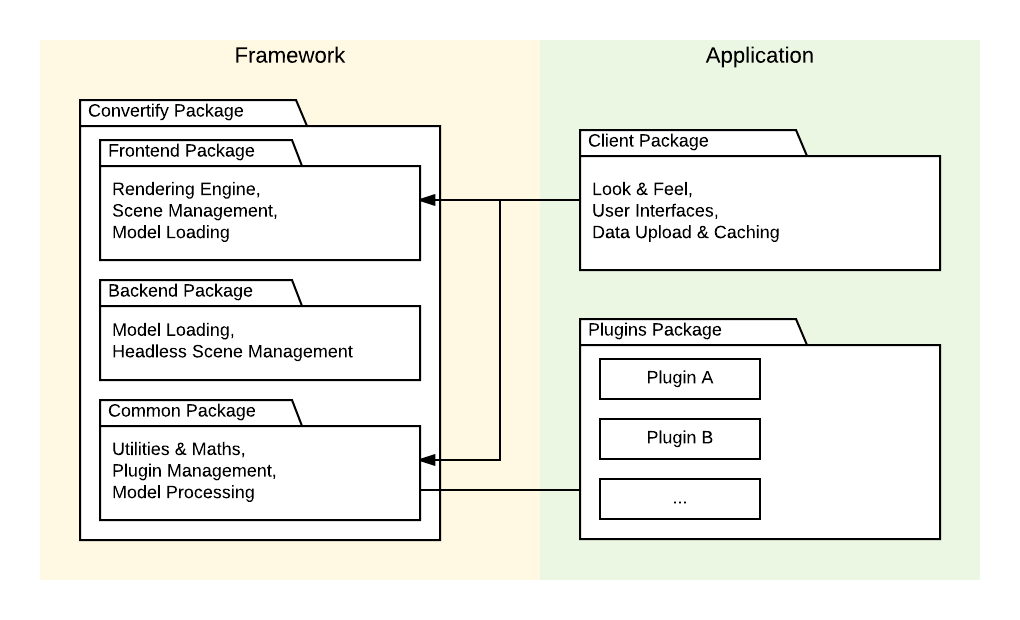
\includegraphics[width=1\textwidth]{03-architecture-package-diagram-overview}
  \caption{Packages of {\convertify}}
  \label{fig:platener-package-diagram-overview}
\end{figure}

We will explain core features of {\convertify} in
Section~\sectionref{sec:convertify-core-features}. Then we will dive into
its plugin system in Section~\sectionref{sec:plugin-system}. {\convertify} is
based on previous work by \citet{bachelor-thesis}. We will give a
short comparison of their work with {\convertify} in
Section~\sectionref{sec:brickify-comparison}. We elaborate on the client
package when we talk about our application {\platener} in
Section~\sectionref{sec:application-platener}.

\subsection{Introduction to the Core System of {\convertify}}
\label{sec:convertify-core-features}

In this section we present the core system of {\convertify}.
{\convertify} helps to build WebGL applications by providing
abstractions to the rendering engine and by composing
features into plugins. We will focus on important design
decisions, which are scene management, rendering and
plugins.

\subsubsection{{\threedmodel}s Are Managed in a Flat Scene
  Graph}

We use a flat scene graph to manage loaded {\stlfile}s. A
flat scene graph has only one level of hierarchy. Such a
graph is sufficient because the {\stlfile}s do not represent
nested models.

We implement the flat scene graph using \class{Nodes}.
\class{Nodes} are abstract objects which represent an entity
in our scene graph. Each \class{Node} references an input
model. The input model is a face-vertex mesh that is either
used for rendering or used by algorithms for further
computation. When the model is used for rendering it is
displayed in the scene. Important parts of the model can be
highlighted. Figure~\ref{fig:vr-glasses:red} shows virtual
reality glasses where the bendable area is highlighted in
red. When the {\threedmodel} is used for computation,
geometries can be analyzed and manipulated.
Figure~\ref{fig:vr-glasses:plates} illustrates computed
plates of the virtual reality glasses.

\begin{figure}[h]
  \centering
  \begin{subfigure}[b]{0.49\textwidth}
    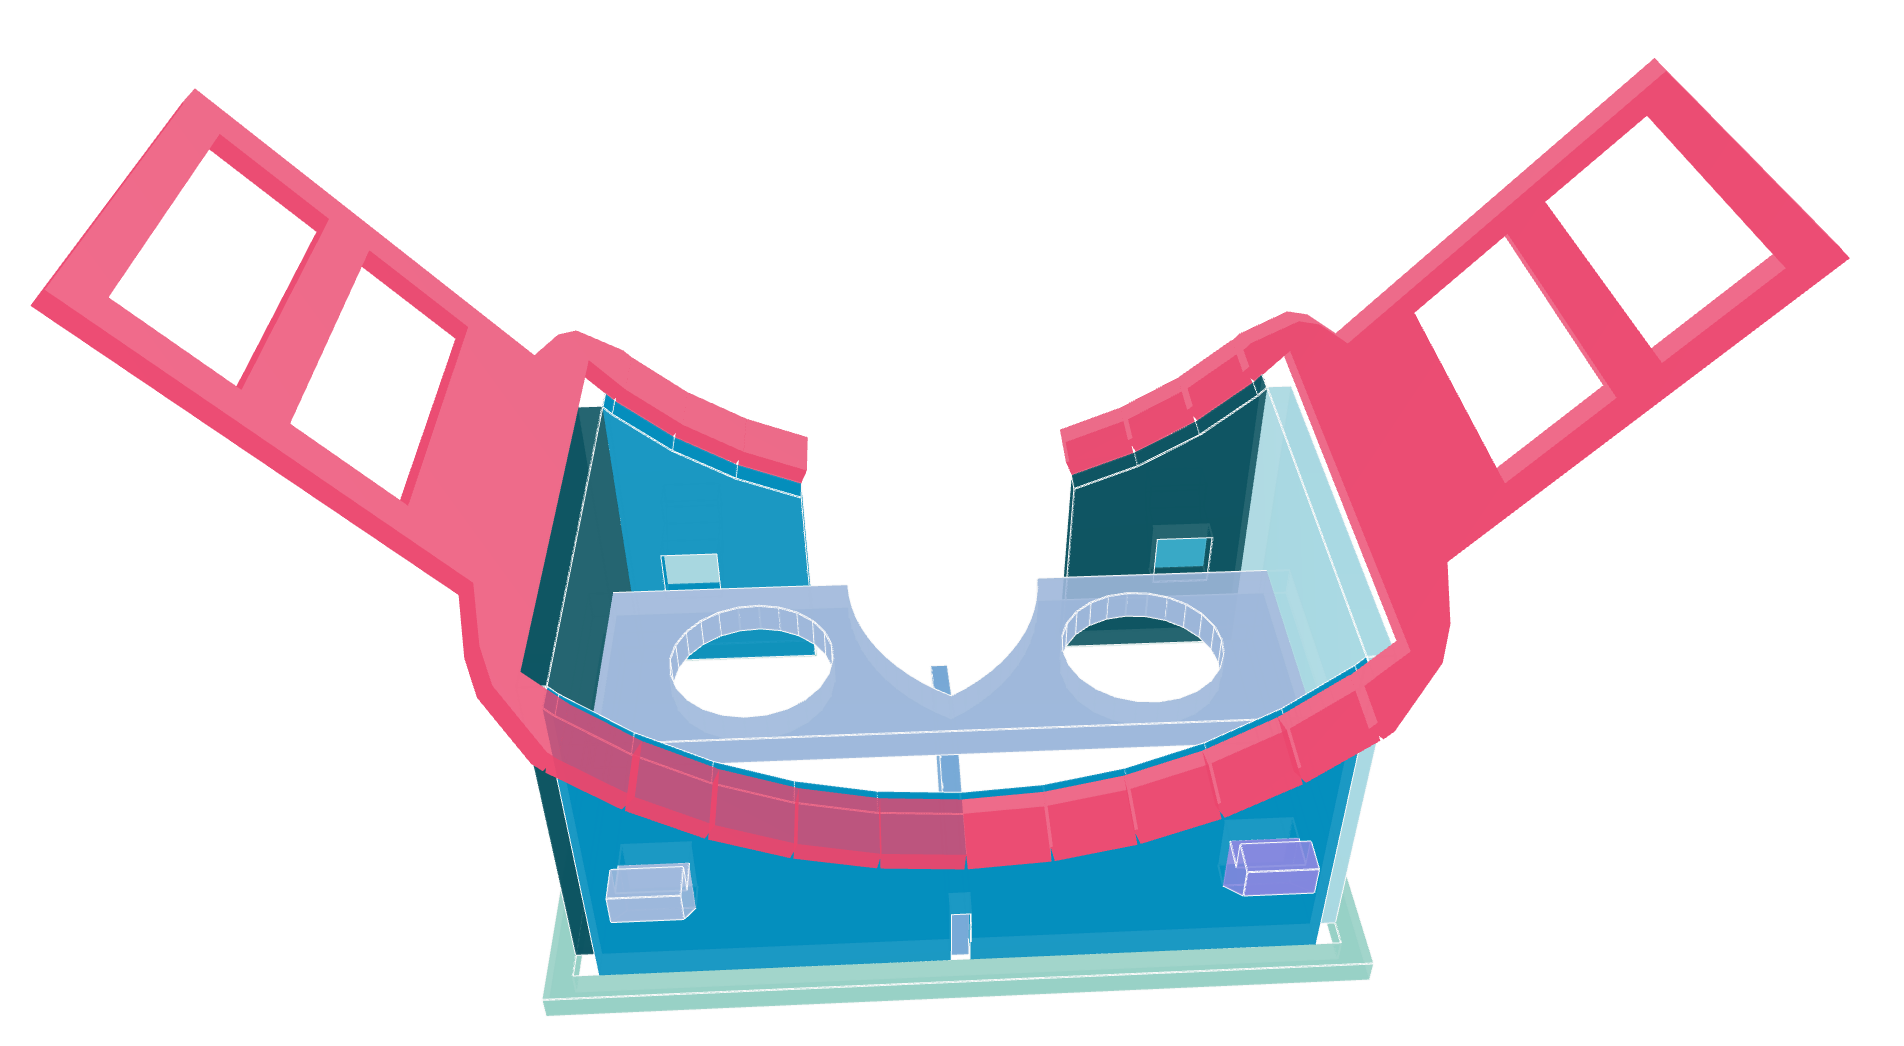
\includegraphics[width=\textwidth]{03-architecture-vr-glasses-red}
    \caption{The bended area is highlighted in red.}
    \label{fig:vr-glasses:red}
  \end{subfigure}
  \begin{subfigure}[b]{0.49\textwidth}
    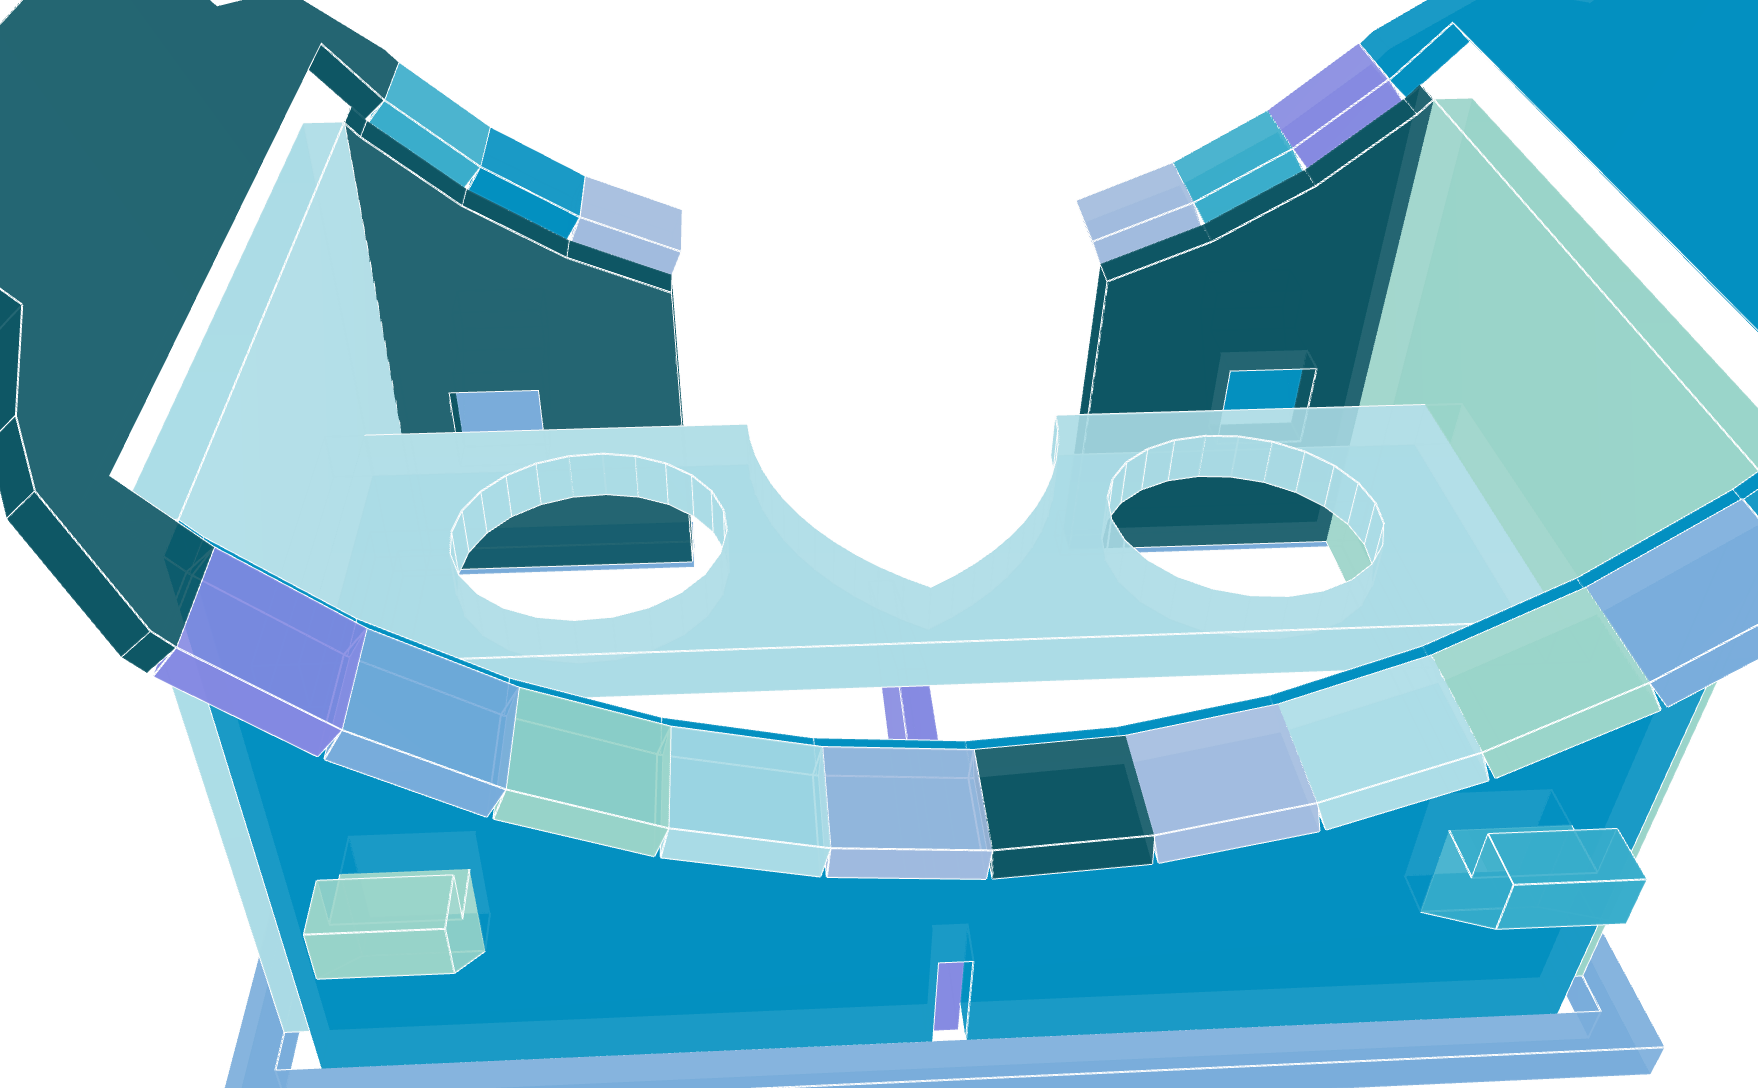
\includegraphics[width=\textwidth]{03-architecture-vr-glasses-plates}
    \caption{Plates are computed by an algorithm.}
    \label{fig:vr-glasses:plates}
  \end{subfigure}
  \caption{The input model are virtual reality glasses.}
  \label{fig:vr-glasses}
\end{figure}

All \class{Nodes} are part of a \class{Scene}.
Figure~\ref{fig:scene-graph} shows how these classes relate.
A \class{Scene} holds references of \class{Nodes}, so we can
access the input models for later usage. \class{Nodes} are
added to or removed from the \class{Scene} via the
\class{SceneManager}.

\begin{figure}[h]
  \centering
  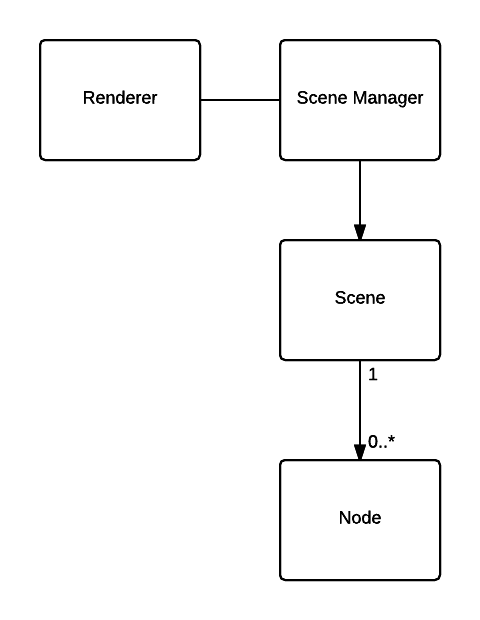
\includegraphics[width=0.6\textwidth]{03-architecture-scene-graph}
  \caption{Relation of scene graph components}
  \label{fig:scene-graph}
\end{figure}

\subsubsection{{\threedobject}s Are Rendered with
  {\threejs}}

In the prior sections we explained that the input data for
{\convertify} is loaded from {\stlfile}s. These
{\threedmodel} representations are stored in face-vertex
meshes and attached to \class{Nodes}.
% A \class{Scene} contains all \class{Nodes} that reference an
% input model.
Though \class{Nodes} represent entities in the scene of
{\convertify}, only {\threejs} objects can actually be
rendered. Such {\threejs} objects are instances of
\class{THREE.Object3D}\footnote{\url{http://threejs.org/docs/\#Reference/Core/Object3D}}.
This is a generic object which can be rendered into a WebGL
scene.
% These \class{THREE.Object3D} will be displayed on the
% screen.
The scene graph of {\threejs} is not flat. A
\class{THREE.Object3D} can have a hierarchy of objects of
any size. Figure~\ref{fig:nodes-and-three} shows the
\class{THREE.Object3D} in the context of \class{Nodes} and
the \class{Renderer}.

We use a \class{Renderer} instance to bring {\threejs}
entities to the screen. The \class{Renderer} sets up a WebGL
context and initializes {\threejs}. In {\convertify} we use
plugins in which we can provide additional features. Plugins
are described in detail in
Section~\sectionref{convertify-emits-events}. We associate each
plugin with a \class{THREE.Object3D} and vice-versa. Thus,
we enable plugins to enhance the scene with new objects. The
\class{Renderer} then traverses the hierarchy of each
associated \class{THREE.Object3D} and renders it.

The \class{Node} contains the input model. A plugin accesses
\class{Nodes} via system events. We explain system events in
Section~\sectionref{convertify-emits-events}. The plugin uses the
\class{Node} to append the input model data to its
associated \class{THREE.Object3D}.


\begin{figure}[h]
  \centering
  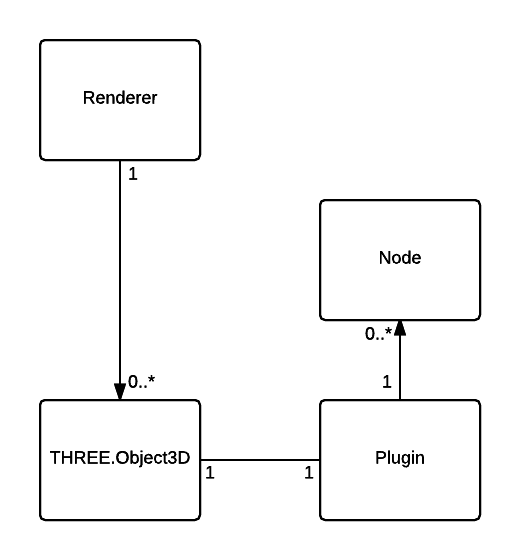
\includegraphics[width=0.6\textwidth]{03-architecture-threejs-objects}
  \caption{\class{Nodes} and indirectly associated \class{THREE.Object3D}}
  \label{fig:nodes-and-three}
\end{figure}

\subsubsection{{\convertify} Emits System Events}
\label{convertify-emits-events}

The framework allows building interactive and modular WebGL
applications. To be capable of interacting with the user,
{\convertify} handles touch and pointer events. As an
application is composed of multiple independent plugins,
these plugins are integrated with the core of
{\convertify}'s system. To realize interactions and
modularity, {\convertify} emits system events during the
loading and render process.

A system event notifies subscribers about changes of the
state of {\convertify} during its lifecycle. Such changes
can be touch or pointer interactions with rendered models in
the scene (\name{onPointerEvent}) or change events to the
scene graph (\name{onNodeAdd}, \name{onNodeRemove}).
Figure~\ref{fig:lifecycle} shows the full lifecycle and
event loop of {\convertify}. Events concerning the scene
management will have the \class{Node} as payload, so plugins
can access the \class{Node}.

\begin{figure}[h]
  \centering
  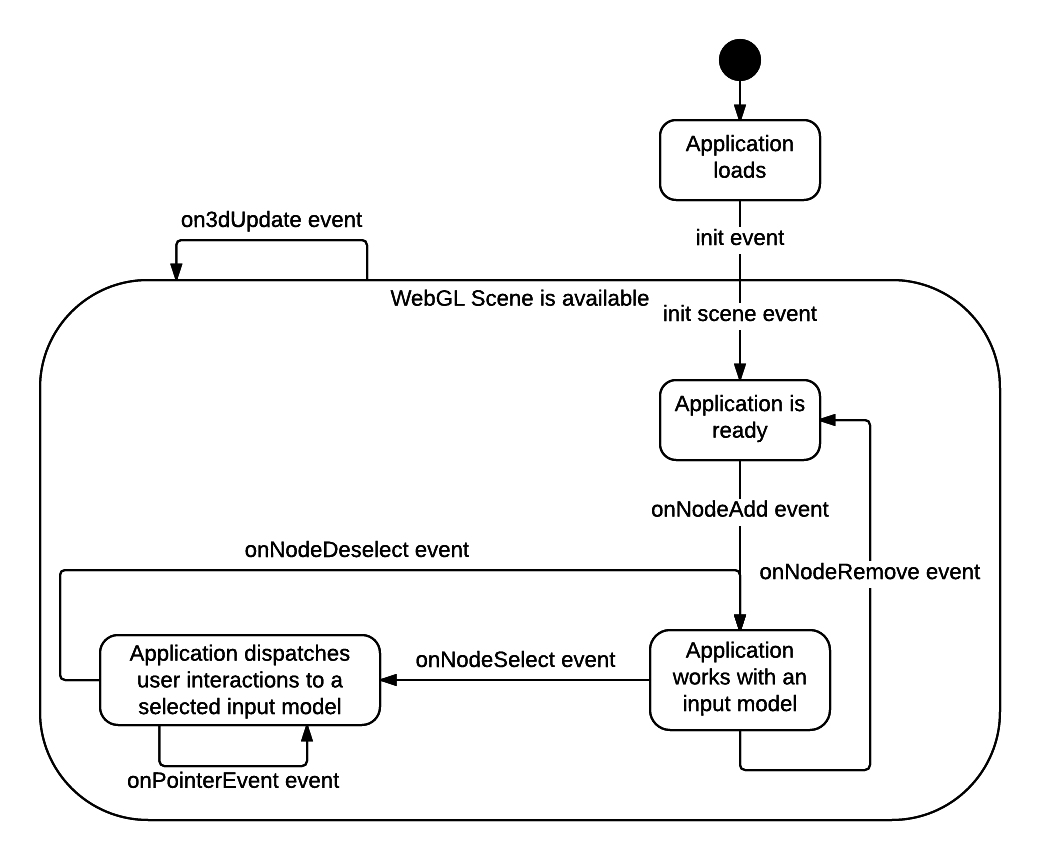
\includegraphics[width=1.2\textwidth]{03-architecture-lifecycle-convertify}
  \caption{The complete lifecycle of {\convertify}}
  \label{fig:lifecycle}
\end{figure}

\subsubsection{{\convertify} Integrates Additional Features
  Via Plugins}

{\convertify} loads additional features into its system via
plugins. Plugins encourage to decompose feature sets into
independent components. A plugin is a separate code package
that contains visualizations for the WebGL scene or
algorithmic computation units. Therefore, it provides a set
of methods which can be called upon emitted system events.
We refer to these callbacks as \class{PluginHooks} or simply
hooks.

\subsection{{\convertify} Provides a Plugin System}
\label{sec:plugin-system}

% - Subsection overview

In this section we present a plugin system that reacts to
{\convertify}'s system events. Additionally, we introduce a
method which organizes communication between
plugins.

% - Plugin definition in Convertify
% - *feature for web gl scene and reaction on changes of the scene*
% - *full fledged applications will implement a set of plugins to
% provide functionality and web ui code to provide interface*

A plugin bundles an exchangeable set of features which will
interact with the WebGL scene or will react on changes to
the scene. Such features are touch interactions with the
rendered model or computations on the model data, triggered
when a \class{Node} is added to the scene. Any full fledged
application implements a set of plugins to provide the scene
functionality. For example, a concrete conversion strategy
provided by {\platener} is implemented by the
\name{PlatenerPipeline} plugin.
Figure~\ref{fig:plugin-constellation} shows our seven
plugins and how they relate to each other. We give an
overview for each plugin in
Section~\sectionref{sec:platener-uses-plugins}.

\begin{figure}[h]
  \centering
  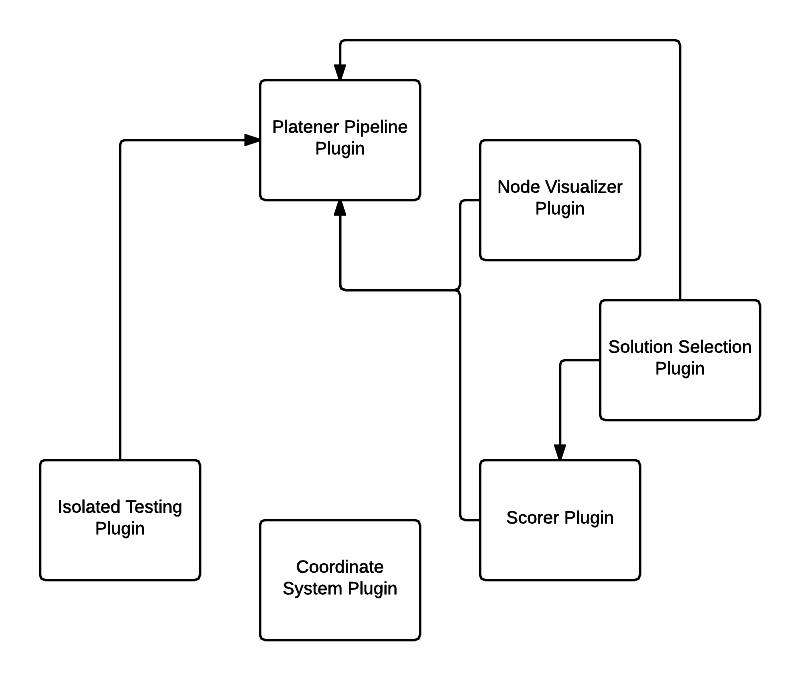
\includegraphics[width=1\textwidth]{03-architecture-plugin-constellation}
  \caption{Platener's plugins and their dependencies.}
  \label{fig:plugin-constellation}
\end{figure}

\subsubsection{Plugins Interact with the Internal System via
  Lifecycle Events}

% - needs-ref :: Lifecycle events in Convertify (= PluginHooks of
% Brickify, Convertify vs. Plugins)
% - needs-figure :: Example Plugin, interacting via PluginHooks
% - System dispatches events (where do events come from?)

{\convertify} emits system events from internal components.
Figure~\ref{fig:lifecycle} depicts the system's lifecycle
and the emitted events. The subscribers to system events are
plugins. Each event can be handled by a
\class{PluginHook} if a plugin implements it. To
implement a \class{PluginHook} each plugin registers
a callback for that event. These callbacks get called when
the event is dispatched by the system. Thus, plugins
can react to each event and apply their own functionality to
the scene or even the model geometry. With this we emphasize
compact computation units in plugins which can still
interact freely with the system.

For better illustration of the functionality of plugins, we
have a look at the \name{PlatenerPipeline} plugin.
Figure~\ref{fig:workflow-platener-pipeline} shows how this
plugin integrates with {\convertify} events. The
\name{PlatenerPipeline} plugin is a plugin implemented for
{\platener}. The plugin reads the model data from a
\class{Node} after a {\threedmodel} was loaded into the
scene. Then it processes the data to create a {\lasercutter}
conversion. Once the model is deleted from the scene by a
user, the plugin releases the processed data. This plugin
does not react to further user interactions, like clicking
or rotating the model.


\begin{figure}[h]
  \centering
  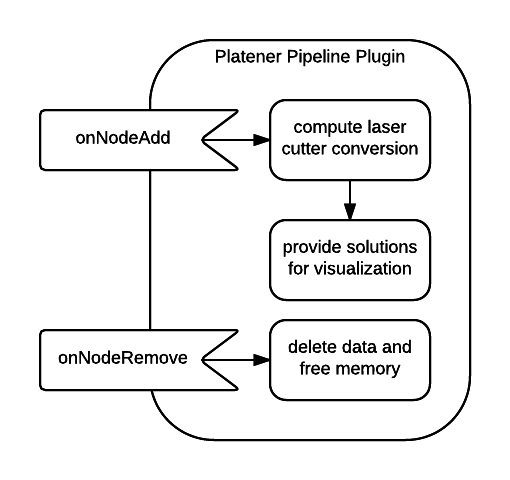
\includegraphics[width=0.6\textwidth]{03-architecture-platener-pipeline}
  \caption{Workflow of the \name{PlatenerPipeline} plugin.}
  \label{fig:workflow-platener-pipeline}
\end{figure}

\subsubsection{Organizing Plugin Communication with a
  Dispatcher}

% - needs-ref :: mediator organizes communication
% - needs-figure :: mediator between dispatched system events and
%                   plugins (internal handling of system events
%                   before reaching plugins)

As {\convertify} manages multiple plugins, which either represent
computation logic or render components, we have to know exactly when
each of these plugins will interact with the system. As
Figure~\ref{fig:plugin-constellation} shows, the dependencies between
plugins are hard to oversee. We propose a \class{Dispatcher}
component, behaving similar to the \name{mediator} pattern.
Figure~\ref{fig:plugin-constellation-with-dispatcher} shows how the
dependencies between plugins are managed with a \class{Dispatcher}.

\begin{figure}[h]
  \centering
  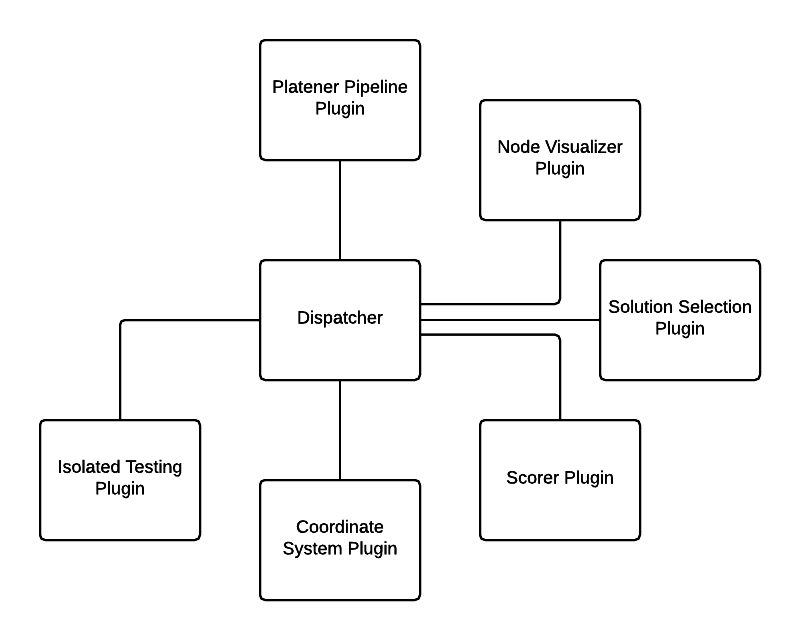
\includegraphics[width=1\textwidth]{03-architecture-plugin-constellation-with-dispatcher}
  \caption{Platener's plugins, managed by a \class{Dispatcher}.}
  \label{fig:plugin-constellation-with-dispatcher}
\end{figure}

According to \citet{gof}, the \name{mediator} pattern is a
behavioral software design pattern. The mediator encapsulates
interconnections of components. It acts as a communication hub and
coordinates its clients. The client components are loosely coupled as
the clients communicate with the mediator instead of communicating
with each other directly. With a mediator we can model many-to-many
relationships \cite[p. 273]{gof}.
% https://sourcemaking.com/design_patterns/mediator

The order of \class{PluginHook} invocations has to be
determined explicitly, because for different events,
different plugins have to run first. For example,
{\platener} wants to process the model data before it is
rendered when a user adds a node to the scene. But it has to
destroy the visualization before releasing all the computed
data. It is not possible to solve the problem by dispatching
all events to all plugins in the same order.

That is why the \class{Dispatcher} implements every
\class{PluginHook}. All system events are emitted to the
\class{Dispatcher} first, before the \class{Dispatcher} will
reemit them to the plugins. This can be seen in
Figure~\ref{fig:dispatching-events}. The \class{Dispatcher}
is a mediator whereas the plugins are the mediator's
clients. With this component in the middle we can control
the order in which the events will be received by the
plugins.

\begin{figure}[h]
  \centering
  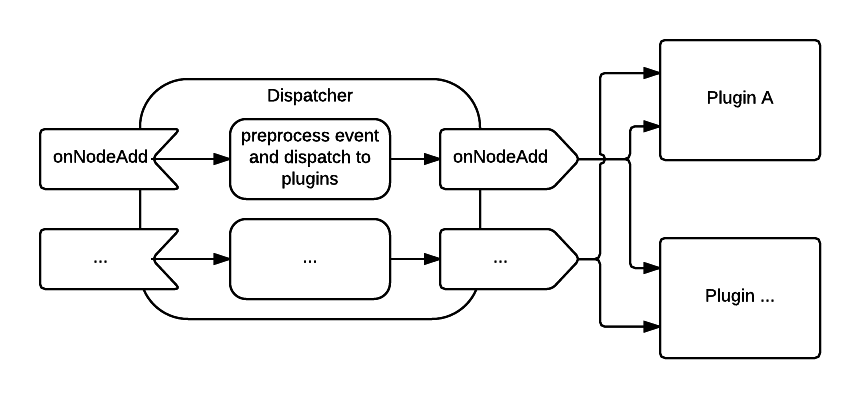
\includegraphics[width=1\textwidth]{03-architecture-dispatching-events}
  \caption{The \class{Dispatcher} remits system events in an explicit order.}
  \label{fig:dispatching-events}
\end{figure}

Plugins are modular feature sets for our applications.
Sometimes it is advisable to separate functionality into
multiple plugins, even if they share the same data. In
{\platener} the \name{PlatenerPipeline} plugin holds all
computed conversions. This plugin does not produce any
visual output. This is necessary as we want to use this
plugin in our CLI tool as well. The \name{NodeVisualizer}
plugin has to read the computed data from the
\name{PlatenerPipeline} plugin in order to displays it.

To model many-to-many relationships between plugins we
enhance the \class{Dispatcher} with \class{Protocols}.
Figure~\ref{fig:protocol-and-plugin} shows how the mediator
connects two plugins. A \class{Protocol} is a mixin
implemented by the \class{Dispatcher}. A mixin adds
functionality to an object by object
composition \cite[p.~81]{js-design-patterns}.
% In
% {\javascript} we realize this with metaprogramming.
A plugin accesses functionality of another plugin by sending
messages to the \class{Dispatcher}. Therefore, the
\class{Protocols} of the \class{Dispatcher} use the
delegation pattern.
% \class{Protocols} define mixins on the \class{Dispatcher}
% which allow delegation of functionality from the
% \class{Dispatcher} to a plugin.
The delegation pattern achieves the results of multiple
inheritance by object composition. It introduces delegating
objects and delegates. A delegating object calls external
functionality on a delegate object which is available
through a predefined interface \cite{delegation-pattern}.
The \class{Dispatcher} is the delegating object and the
plugin is the delegate.
% The \class{Protocol} helps to define
% the interface between the \class{Dispatcher} and a plugin.
% Two plugins now communicate with each other via the
% \class{Dispatcher}. One plugin calls functionality on the
% \class{Dispatcher} which was exposed by a \class{Protocol}.
The \class{Protocol} ensures that the \class{Dispatcher}
delegates an action to another plugin.
% http://best-practice-software-engineering.ifs.tuwien.ac.at/patterns/delegation.html
% https://developer.apple.com/library/ios/documentation/General/Conceptual/DevPedia-CocoaCore/Delegation.html

\begin{figure}[h]
  \centering
  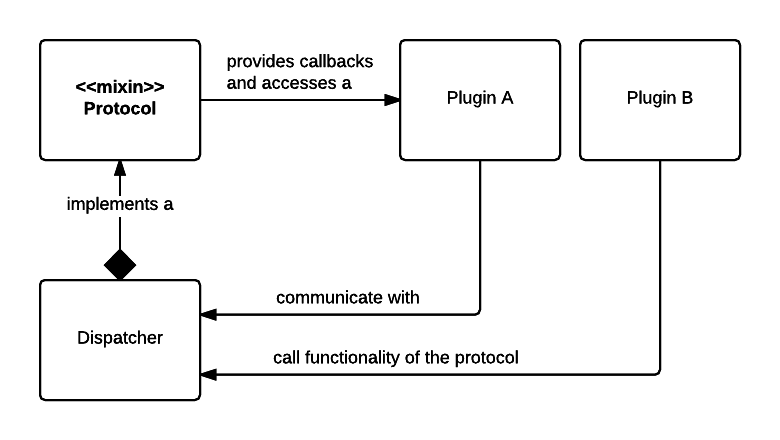
\includegraphics[width=1\textwidth]{03-architecture-protocol-and-plugin}
  \caption{Plugin~B can use features of Plugin~A by calling functionality of the \class{Protocol} implemented by the \class{Dispatcher}.}
  \label{fig:protocol-and-plugin}
\end{figure}

When applications grow it is hard to observe all messaging
between components at once. With the \class{Dispatcher}, we
wire up all communication with plugins in one place. Due to
explicit ordering of callback executions we have
fine-grained control for each plugin. \class{Protocols}
define clean interfaces for plugin communication.

% Each application implemented with
% the {\convertify} framework has to implement a custom
% \class{Dispatcher}.

% - *full fledged applications will implement a mediator to organize
% feature communication*

\subsubsection{A \class{Bundle} Is the Entry Point for Applications Using {\convertify}}
\label{sec:bundle-entry-point}

Setting up a framework typically requires configuring an
entry point. A \class{Bundle} is the entry point for
applications that use {\convertify}, e.g {\platener} uses
the \class{Bundle} to initialize the web application with
{\convertify}'s WebGL scene. The \class{Bundle} is a
controller for {\convertify}. It loads models into the
system and exposes controls for the scene. With this we can
animate the scene programmatically or sync scenes of
multiple {\convertify} instances. The framework requires a
\class{Bundle} for both, frontend and backend package,
because data is accessed differently in browser
environments and {\nodejs}.

% {\convertify} provides a \class{Bundle} instance for its
% frontend and backend packages.

In the preceding section, we introduced a \class{Dispatcher}, which
organizes the communication between plugins and {\convertify}. As
{\convertify} is a framework, multiple applications can be realized
with it. Now, every application wants to organize its plugins and
event handlers differently. That is why each application implements
its own \class{Dispatcher} instance. The \class{Bundle} can be
configured with such a \class{Dispatcher}.
Figure~\ref{fig:bundle-dispatcher} shows the \class{Bundle} in the
context of an application.

\begin{figure}
  \centering
  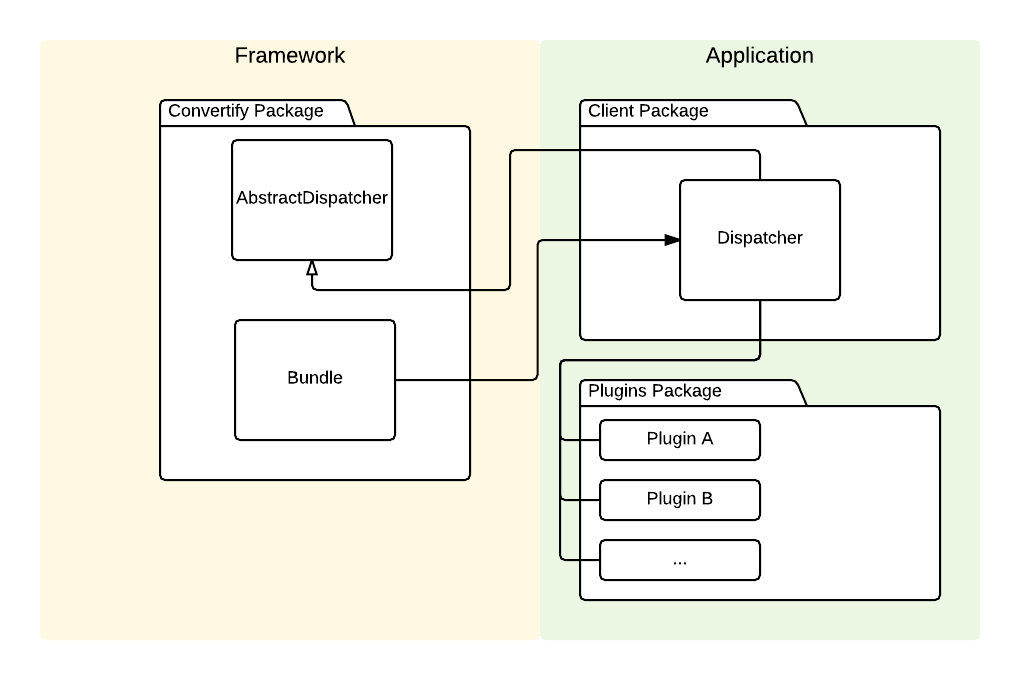
\includegraphics[width=1.1\columnwidth]{03-architecture-bundle-dispatcher}
  \caption{A \class{Bundle} is configured with a \class{Dispatcher}.}
  \label{fig:bundle-dispatcher}
\end{figure}

% whats a bundle
% bundle class

% have it for frontend/ backend package (because loading files etc. is different in browser/ nodejs)
% entry point, initialized with a dispatcher. dispatchers are written in application code.
% so convertify behavior configured via bundle through custom dispatcher.

% why have a bundle?

% give controller for convertify eco system, used by applications, e.g platener
% easy customization -> e.g. synching scenes of multiple instances of convertify -> animations/ controls/ loaded models


\subsection{{\convertify} Is a Cross-platform Isomorphic Framework}
\label{sec:convertify-is-isomorphic}

{\convertify} is a cross-platform framework. {\javascript}
code does not run seamlessly in multiple browsers out of the
box. The code has to be aware of their different
implementations and APIs.
%This allows {\convertify} to run on almost any device.
To enable cross-platform {\javascript} support we use
polyfills and libraries that are cross-platform as well.

Legacy {\javascript} engines do not support data structures
like \class{Map}, \class{Set} or \class{Promise}. We provide
these features with the
\name{es6-shim}\footnote{\url{https://github.com/paulmillr/es6-shim}}
polyfill. A polyfill is \enquote{a piece of code or plugin
  that provides technology that [we] expect the browser to
  support
  natively}\footnote{\url{https://remysharp.com/2010/10/08/what-is-a-polyfill}}.

Using libraries that have cross-platform support themselves enables us
to maintain {\convertify} as a cross-platform framework. Such
libraries are for example
\name{lodash}\footnote{\url{http://lodash.com}} or {\threejs}.
\name{lodash} provides functional utilities which greatly improve the
way we work with our data structures. {\threejs} is the 3D library
which we use for WebGL rendering. The WebGL API is not consistent for every browser
\footnote{\url{https://docs.unity3d.com/Manual/webgl-browsercompatibility.html}}.


{\convertify} is an isomorphic framework. We speak of
isomorphic {\javascript} code when the code can be
seamlessly executed in browser environments and non-browser
environments\footnote{\url{http://nerds.airbnb.com/isomorphic-javascript-future-web
    apps/}}.
% The most common non-browser {\javascript}
% environment is {\nodejs}\footnote{\url{https://nodejs.org}}.
{\convertify} can use its full feature set in {\nodejs}.
This enables us to write applications that can be integrated
into other environments or workflows. In the case of our
application {\platener} we can batch process 3D-models from
a command line interface. The CLI is described in
Section~\sectionref{sec:cli-tool}.

% \note{explain isomorphic = headless}
% \note{explain what
%   convertify can do when isomorphic}
% \note{explain how convertify is
%   isomorphic}
% \note{explain why convertify is isomorphic (pros)}


\subsection{{\convertify} Is Built on {\brickify}}
\label{sec:brickify-comparison}

The web application {\brickify} was introduced in
Section~\sectionref{sec:related-work}. {\brickify} provides several
features that we reuse for {\convertify}. We integrate the
rendering engine with its scene management and event system.
We greatly improve the event system by using a
\class{Dispatcher}. Also, {\brickify} provides the basic
functionality of our plugin system. Though we enhance plugin
communication via \class{Protocols}. In general {\brickify}
combines {\userinterface} elements with its logic
components. With {\convertify} we have a modular framework
that is completely decoupled from any {\userinterface} code.

\subsection{A Variety of Possible Applications Can Be Built with the {\convertify} Architecture}
\label{sec:variety-of-applications}

Based on {\brickify}'s groundwork and our improvements to
the system, we provide a set of common functionality which
is useful for any web based 3D application. We focus on
3D-Models as primary data representation. We enable users to
perform customization to these models in real-time. The
computed results are visualized for the user. We support
cross-platform browsers using WebGL technology. We allow
mouse and touch interactions with the scene. This enables
users to interact with {\convertify} from desktop or mobile
systems. As {\convertify} is fully isomorphic its
applications can be integrated into other software by
packaging the code as an independent {\nodejs} module.

\end{document}

%%% Local Variables:
%%% mode: latex
%%% TeX-master: "../../ClassicThesis"
%%% TeX-command-extra-options: "-shell-escape"
%%% End:
